\chapter{Konstruktion}

Die Konstruktion des E-Bikes begann mit einer gründlichen Analyse der benötigten Komponenten und deren Positionierung, einschließlich der Batterie, des Motors und des Controllers.
Um die optimale Platzierung zu ermitteln, wurde zunächst ein Test mit einem verfügbaren Laufrad durchgeführt, welches sich als geeignete Testplattform erwies.

\section{Positionierung der Komponenten}

Für den Antrieb wurde zunächst ein Frontantrieb in Betracht gezogen und getestet, dies führte jedoch zu unerwünschtem Durchdrehen des Rades, selbst bei geringer Leistung von nur 50\%.
Daraufhin wurde die Batterie in der Mitte des Rahmens positioniert, um eine gleichmäßige Gewichtsverteilung zu gewährleisten,
dies erwies sich dynamischer, als auch aus statischer Sicht vorteilhafter.
Siehe Bild~\ref{fig:27}.
\begin{figure}[h!]
    \centering
    \includegraphics[width=8cm]{images/Bild des Laufrads}
    \caption{Laufrader Test\cite{lorenz_scherrer_selbst_2023}}
    \label{fig:27}
\end{figure}


Schließlich wurde die Entscheidung getroffen, den Motor am Hinterrad anzubringen, und die Batterie weit vorne am Rahmen zu platzieren, um das Gewicht auszubalancieren, insbesondere aufgrund des schweren Hinterradantriebs. 
Der Controller wurde an der hinteren Flaschenhalterung montiert, dies erweist als funktional.
Der Controller und das gesamte Fahrrad sind in Abbildung\ref{fig:28} zu sehen.


\begin{figure}[h!]
    \centering
    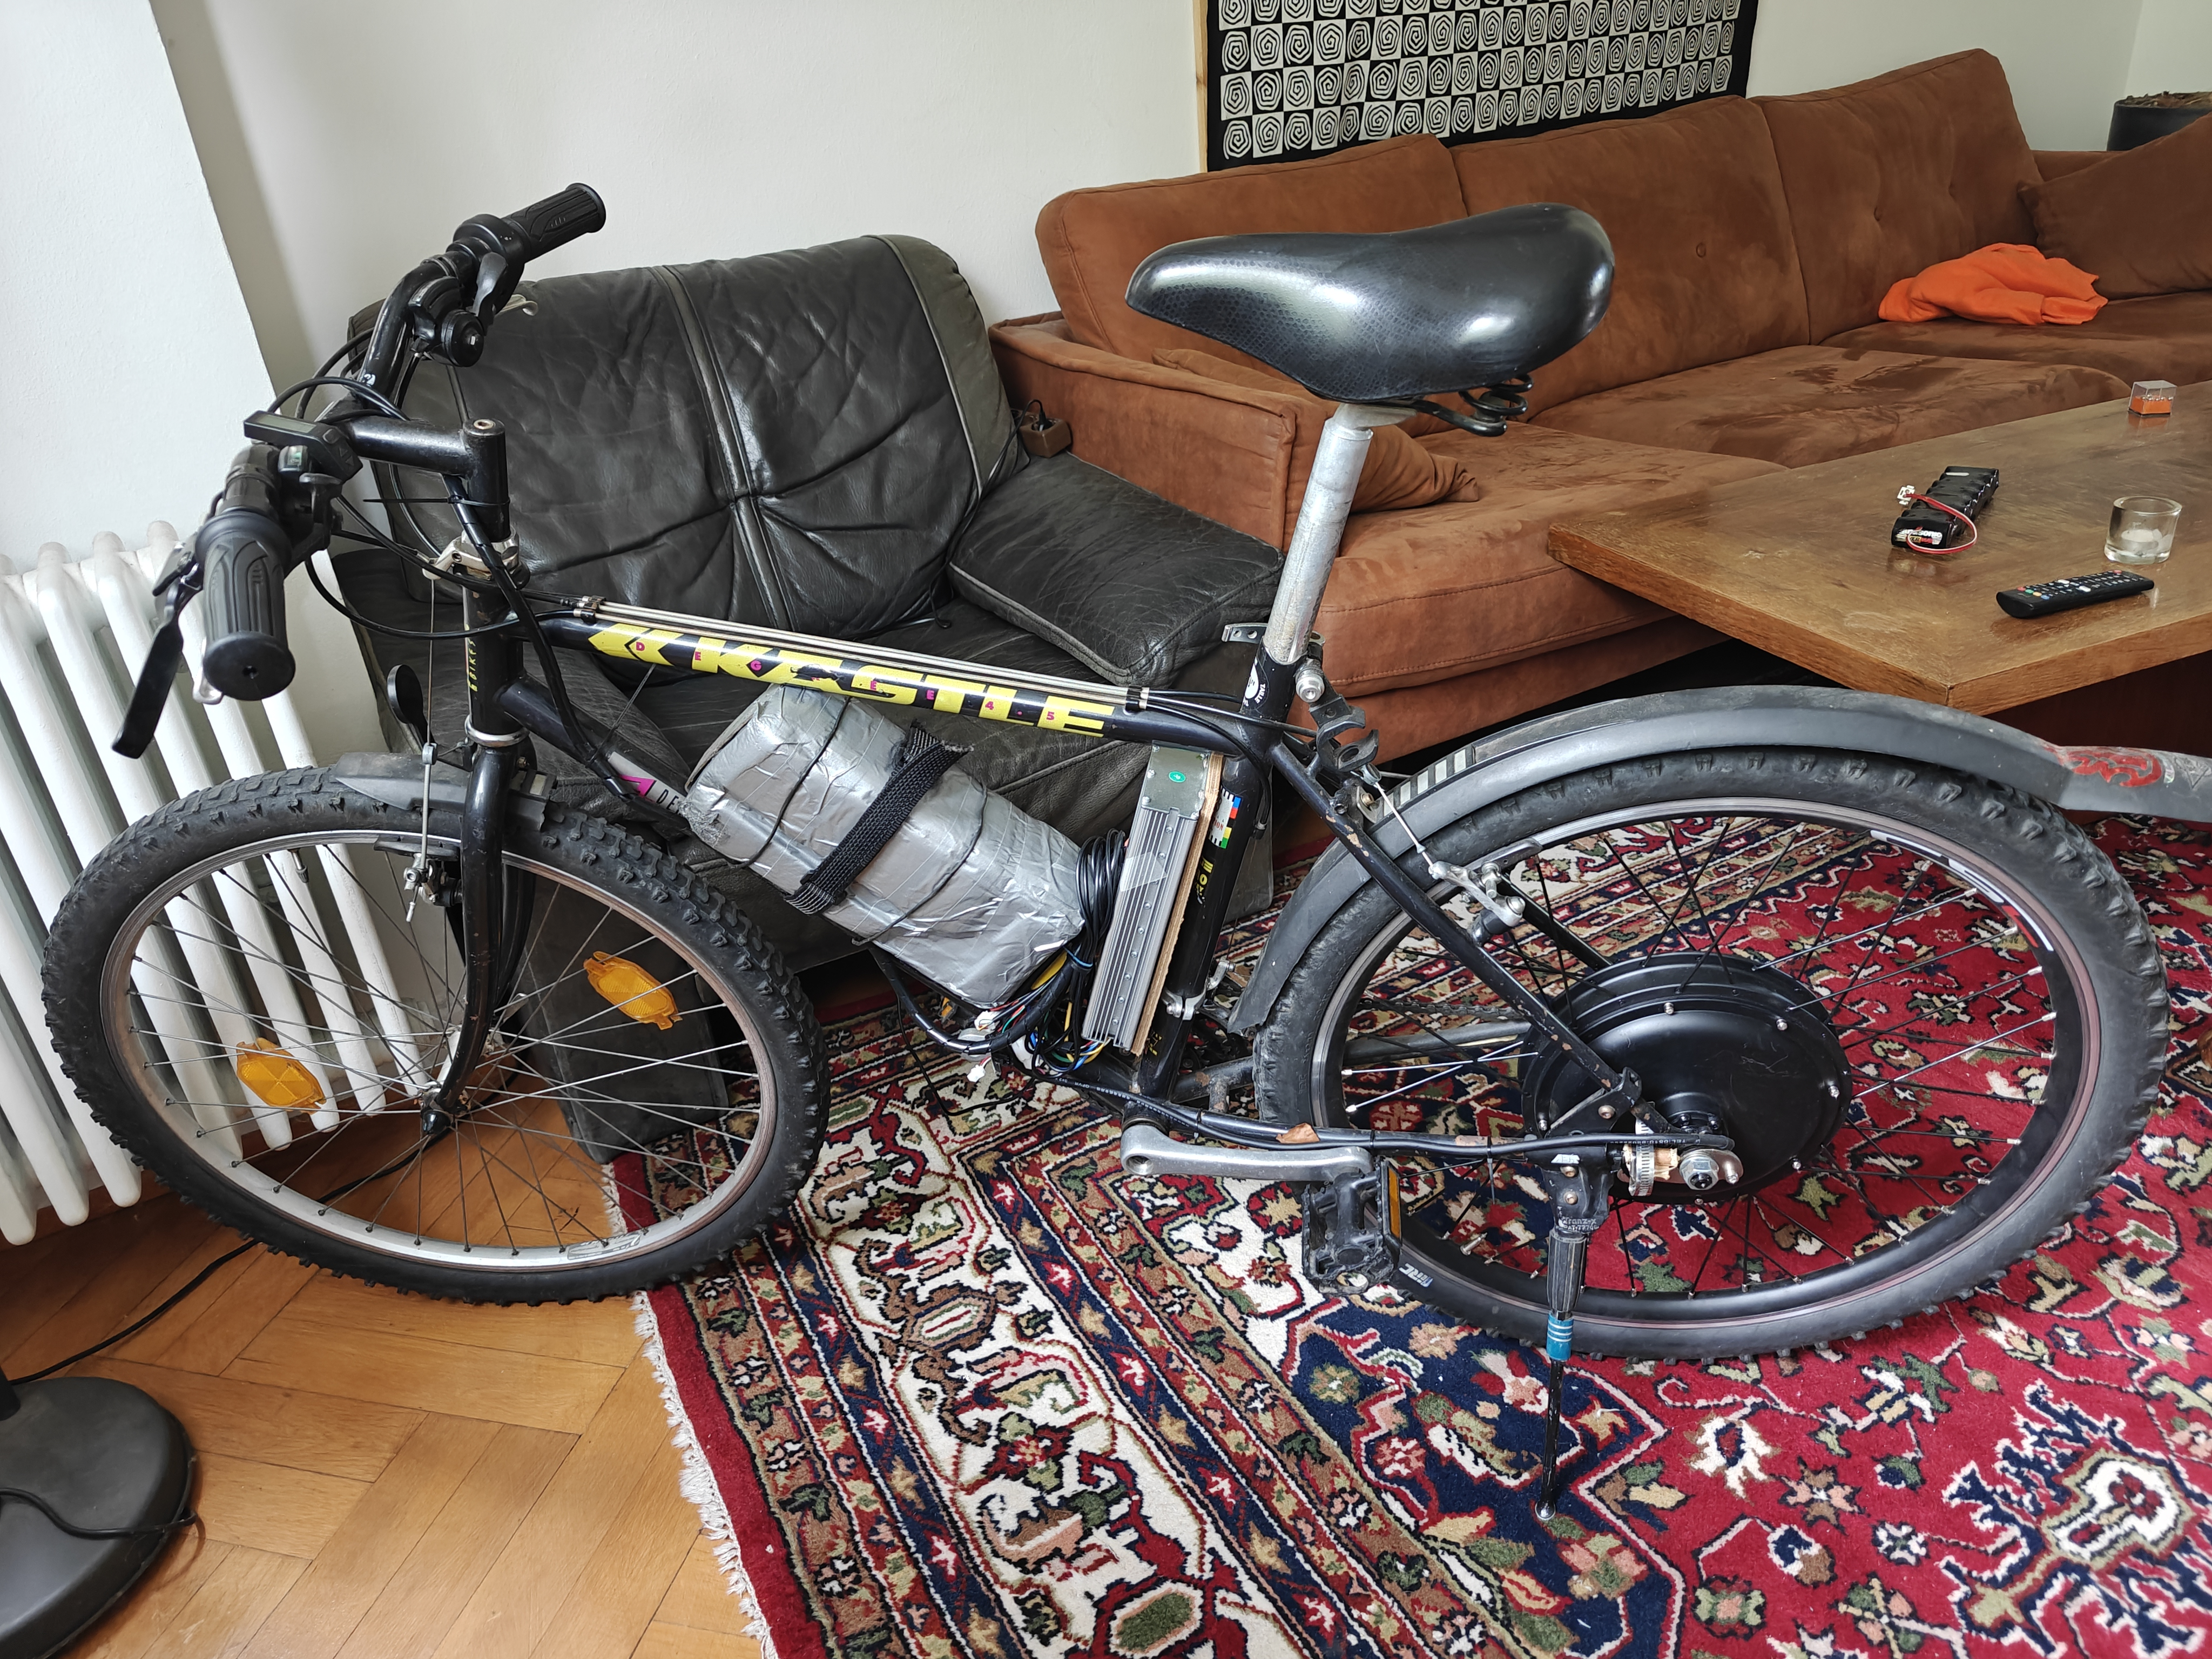
\includegraphics[width=8cm]{images/Bild des Fahrrads}
    \caption{Kompletes Fahrrad\cite{lorenz_scherrer_selbst_2023}}
    \label{fig:28}
\end{figure}


Für die Befestigung der Batterie wurde robustes Stahlblech verwendet, das sorgfältig gebogen und mit einer Schlaufe gesichert wurde.
Dieser Bügel wurde am vorderen Getränkehalter angebracht, um das Gewicht gleichmäßig zwischen dem Hinterrad-Antrieb zu verteilen.
Obwohl diese Befestigungsmethode sich als nicht ganz stabil erwies und die Batterie während des Tests herunterfiel, konnte sie dennoch vorübergehend gesichert werden.
Im nachfolgen Bild\ref{fig:29} ist die Montage dargestellt.
\begin{figure}[h!]
    \centering
    \includegraphics[width=8cm]{images/Bild der Batterie am Fahrrad}
    \caption{Batterie montiert\cite{lorenz_scherrer_selbst_2023}}
    \label{fig:29}
\end{figure}


Die Verkabelung erfolgte anschließend.
Wobei die Bremsen durch elektrische Bremsen ersetzt wurden, das Drehgas und das Display hinzugefügt wurden.
Die Kabelführung wurde mit einem Spiralkanal und Kabelbindern umgesetzt.
Es wurde darauf hingewiesen, dass der PSA-Sensor während des Projekts nicht hinzugefügt werden konnte~\ref{fig:28}.






\section{Montage des Motors}


Die Montage des Motors erfolgte im Anschluss an die Positionierung der Batterie und des Controllers. 
Ein wichtiger Schritt dabei war die korrekte Befestigung der Motorachse.
Es wurden zwei Muttern verwendet, die fest angezogen wurden. 
Allerdings stellte sich heraus, dass insbesondere bei leistungsstarken Motoren mit einer Leistung von 1500 Watt, die Belastung für die Achse zu hoch sein kann.
Das aufgebaute Drehmoment kann dazu führen, dass die Achse bricht. 
Aus diesem Grund wurde ein Torque Arm verwendet, um die Achse zu verstärken. 
Eine visuelle Darstellung dieses Vorgangs ist im Bild unten dargestellt~\ref{fig:30}.

\begin{figure}[h!]
    \centering
    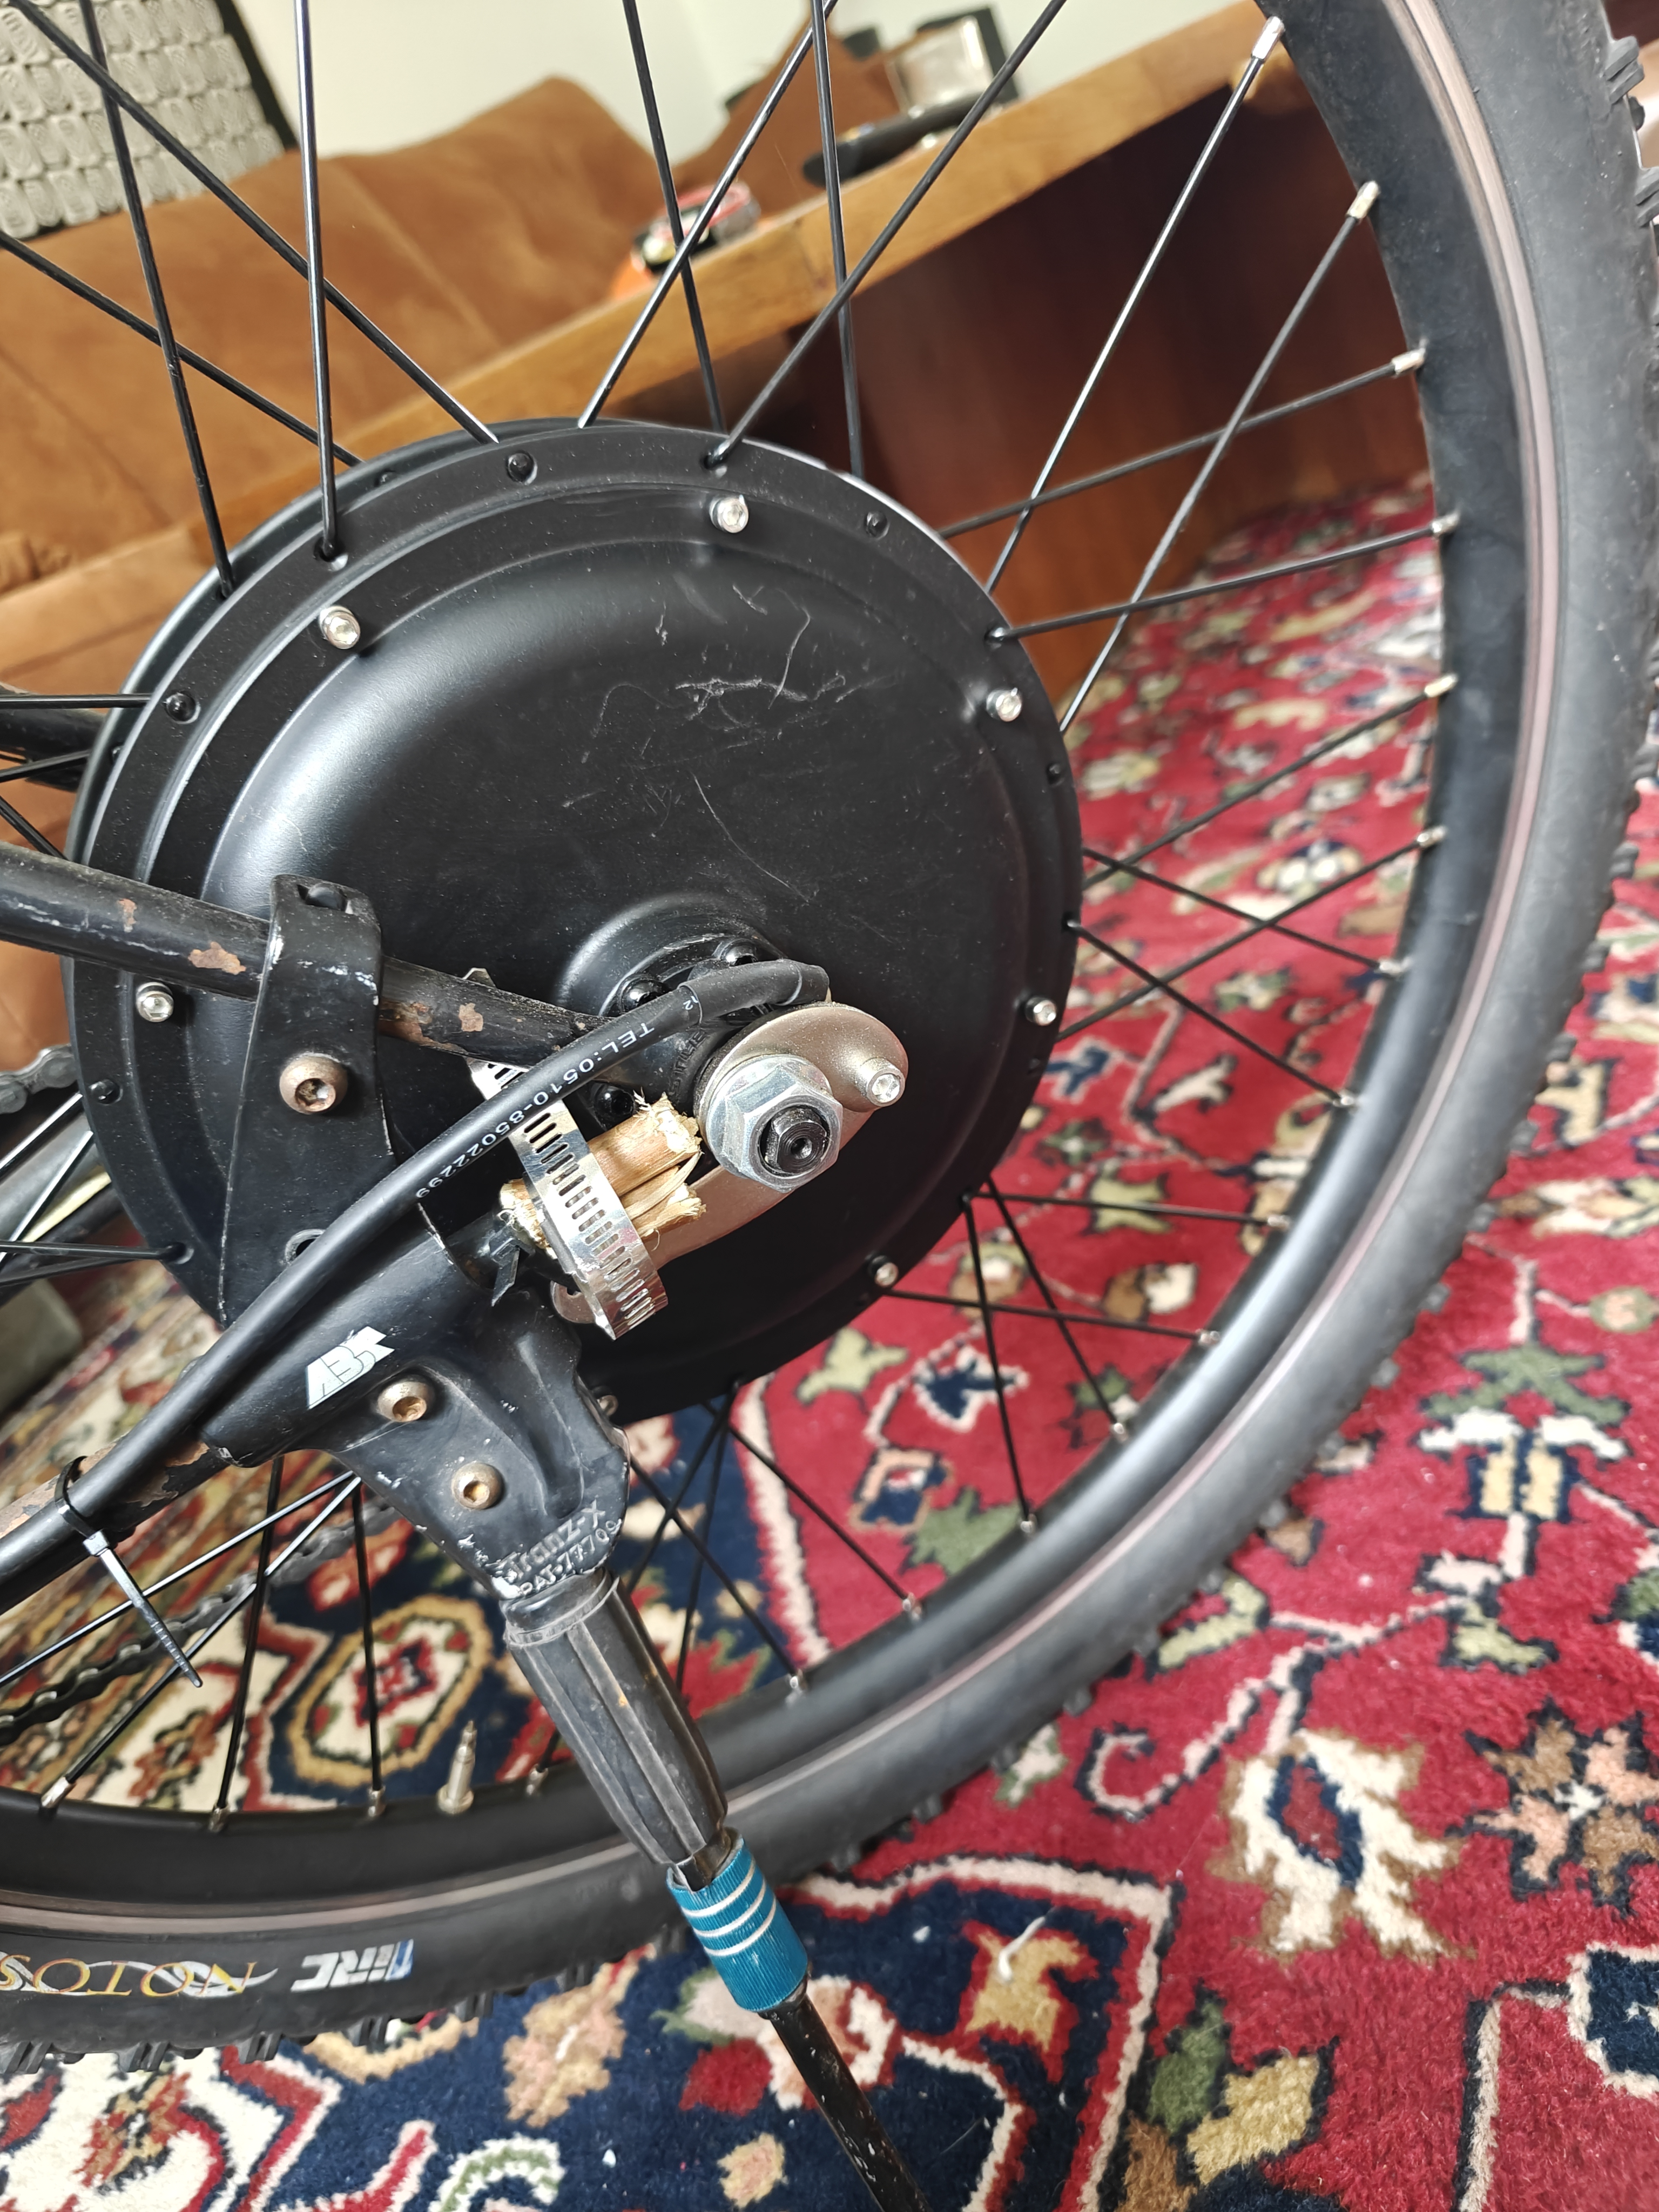
\includegraphics[width=8cm]{images/Bild des Motors}
    \caption{Motor montiert\cite{lorenz_scherrer_selbst_2023}}
    \label{fig:30}
\end{figure}


Die Befestigungsschlaufe erwies sich als etwas zu dünn, weshalb zusätzliche Stäbe eingefügt wurden, um die Stabilität zu erhöhen.
Trotz dieser Anpassungen funktionierte die Montage des Motors insgesamt gut.
Die Bremsbacken mussten an die Felge angepasst werden, wobei festgestellt wurde, dass die Rekuperationsbremse deutlich stärker ist als die konventionelle Bremse.
Dies erwies sich als vorteilhaft, um die letzten Kilometer pro Stunde zu reduzieren, vornehmlich bei niedrigen Geschwindigkeiten, bei der Rekuperationsbremse nicht mehr so effektiv ist.
Dennoch erwiesen sich die Bremsbacken als effektiv und wurden sowohl vorne als auch hinten entsprechend angepasst.
